\chapter{Structure generation}

\section{Chosen approach}

In order to reconstruct the tip shape via ray tracer method, which is an innovative way to simulate and reconstruct the tip, an ideal image of the measured sample has been generated. To this purpose, an ideal point-shaped tip has been considered and approximated by means of a monoatomic tip or a Dirac's delta shaped tip. Thus, the simulation of the ideal measurement has been performed by computing the height of each pixel by using \textit{z-test} (or \textit{depth-test}) technique \cite{raycasting_ztest}, that is commonly used in ray tracers. In particular, \textit{z-test} relies on testing the distance between a given point and the planar camera and, if another point that should be drawn in the same pixel is closer, the algorithm substitutes the previous one. (see Fig. \ref{fig:concept}). This will ensure a correct occlusion handling.

\begin{figure}[ht]
    \centering
    %  concept
    \includegraphics[width=.95\textwidth]{./immagini/concept.png}
    \caption{Ray Tracer z-test method}
    \label{fig:concept}
\end{figure}

\newpage

The constant evolution in terms of performances, due to ever-improving hardware and dedicated programming languages, makes raytracers advantageous \cite{GPU_language}. In fact, the field of ray tracing has made significant progress in recent years, with improvements in rendering speed, accuracy, and efficiency, largely driven by the use of powerful graphics processing units (GPUs). The ability to simulate ideal measurements and accurately reconstruct tip shapes using ray tracing techniques opens up new possibilities for improving the precision and speed of tip reconstruction algorithms in AFM studies.

\section{Models and nanoparticles}

The general method used to create different structures is based on the generation of meshes made of triangles using some known dimensional parameters. Besides z-test, ray tracers usually will perform other shader calculation in order to create photorealistic images. For this project, we will borrow just the algorithm for correctly rendering triangles and their occlusions \cite{raytracer1,raytracer2}.

\vspace{10pt}

Since the coordinates of the mesh triangles are known \textit{a priori}, we can further speed up the calculations by employing a technique called rasterization and fragment processing. This technique calculates the height at a specific point from an interpolation of the three vertices of the triangle in which the point is enclosed using its barycentric coordinates \cite{rasterization}.

\vspace{10pt}

We can create a standard and normalized model of each structure we want to study (spheres, cubes, steps, etc.) with open source or external 3D modelling programs (e.g. Blender \cite{blender}). Hence, given an input of parameters, we can generate the model of the correct size, orientation and position using scale, rotation and traslation matrices. In this way, we can generate an array of triangles that will be resulting in the ideal structure, composed of multiple nanoparticles without resorting to mathematical modelling of the surface.

\vspace{10pt}

In the following sections we will explain all the steps needed to perform the operations starting from the triangle meshes to obtain the final ideal topography.
It is worth knowing that this work focuses on the union of two very broad and different fields. In the future, there will be the possibility to generate the mesh from scratch, while for now, we begin our studies from pre-calculated models. Future routines will also be able to adapt and generate models for more complex geometries and from a base set of written instructions.

\newpage

\section{Triangles}

\paragraph{Barycentric coordinates: }

Every single model that will be generated and simulated will be structured from triangles. This means that we can extract various attributes using barycentric coordinates as shown in Fig. \ref{fig:bary_a} and \ref{fig:bary_b}. Using this method we can define an information of interest (such as depth) at the vertices and interpolate them to obtain a smooth final image as shown in Fig. \ref{fig:bary_b}.

\begin{figure}[ht]
    \centering
    \begin{subfigure}[b]{0.45\textwidth}
        % bary1
        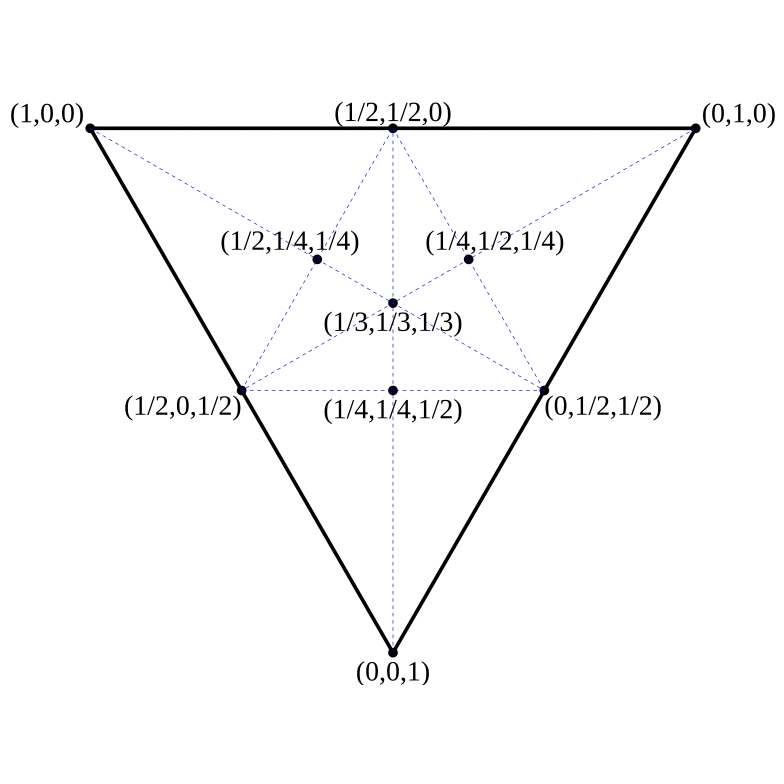
\includegraphics[width=.95\textwidth]{./immagini/bary1.png}
        \caption{}
        \label{fig:bary_a}
    \end{subfigure}
    \hfill
    \begin{subfigure}[b]{0.45\textwidth}
        % bary2
        \includegraphics[width=.95\textwidth]{./immagini/bary2.png}
        \caption{}
        \label{fig:bary_b}
    \end{subfigure}
    \caption{a) Geometrical construction, b) smooth interpolation of baricentric coordinates}
    \label{fig:bary}
\end{figure}

Notice that this process is applied to each triangle that composes the model, thus leading to a heavy computation very quickly. In this case the parallelised computation of powerful graphics processing units (GPUs) proves useful.

\paragraph{Depth test and overalapping:} Once we have more than one triangle there might be overlapping, and to address this issue, we use a ray-tracer simulating technique to test how far a triangle is respect to the camera. In this way we can correctly identify which triangle should actually be part of the simulated nanostructure, see Fig. \ref{fig:depth}. This process will be speed up incredibly by using the standard graphical pipeline used in the video-games industry, backed up by the physical and mathematical correctness of the ray-tracer approach. 

\vspace{10pt}

Hence, by means of this method, we can correctly simulate the nanoparticles discussed in the following chapters.

\newpage

\begin{figure}[ht]
    \centering
    \begin{subfigure}[b]{0.32\textwidth}
        % depth
        \includegraphics[width=.95\textwidth]{./immagini/depth.png}
        \caption{}
        \label{fig:depth_a}
    \end{subfigure}
    \hfill
    \begin{subfigure}[b]{0.32\textwidth}
        % depth2
        \includegraphics[width=.95\textwidth]{./immagini/depth2.png}
        \caption{}
        \label{fig:depth_b}
    \end{subfigure}
    \hfill
    \begin{subfigure}[b]{0.32\textwidth}
        % depth3
        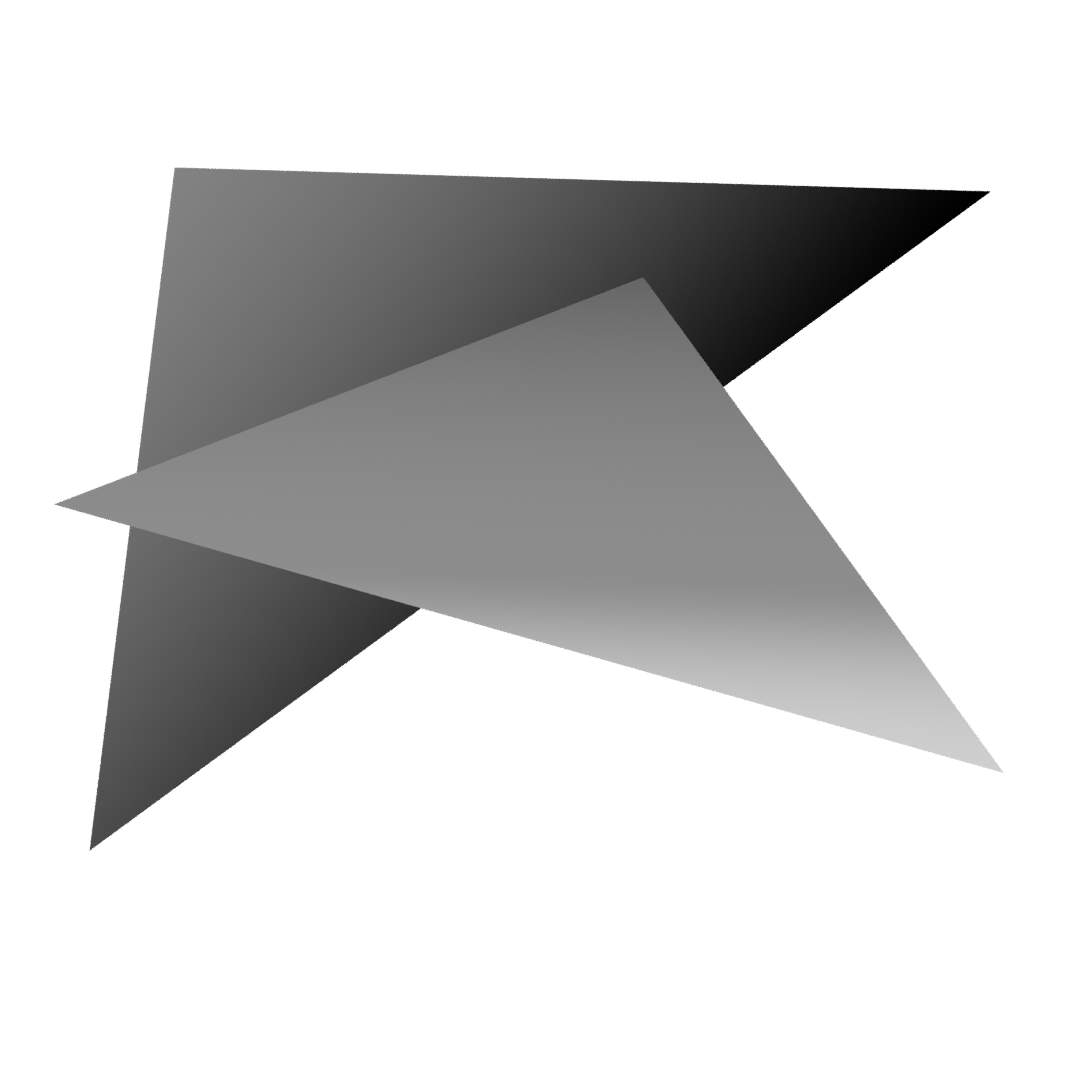
\includegraphics[width=.95\textwidth]{./immagini/depth3.png}
        \caption{}
        \label{fig:depth_c}
    \end{subfigure}
    \caption{a) A pair of triangles of unknown Z height b) Zoom of the overlapping surface c) Final result, obtained from comparing the depth at which each pixel is located}
    \label{fig:depth}
\end{figure}

\section{Spheres}

The standard model is created in Blender using an icosphere with 5 subdivisions. It is centred in the origin with radius r equal to 1.
Then, it is translated by a vector v = (x, y, z) to it is new position and scaled of a given factor in order to match the desired position and dimension. The z-traslation equals to r/2, in order to place the base of the sphere on the floor. This ensures that the nanoparticle rests perfectly on the substrate.
Some examples of generated images are reported in Fig. \ref{fig:sphere}a-c. In particular, Fig. \ref{fig:sphere_b} and \ref{fig:sphere_c} show also compenetrated spheres that are successfully handled by this system.

\begin{figure}[ht]
    \centering
    \begin{subfigure}[b]{0.32\textwidth}
        % sfera_singola
        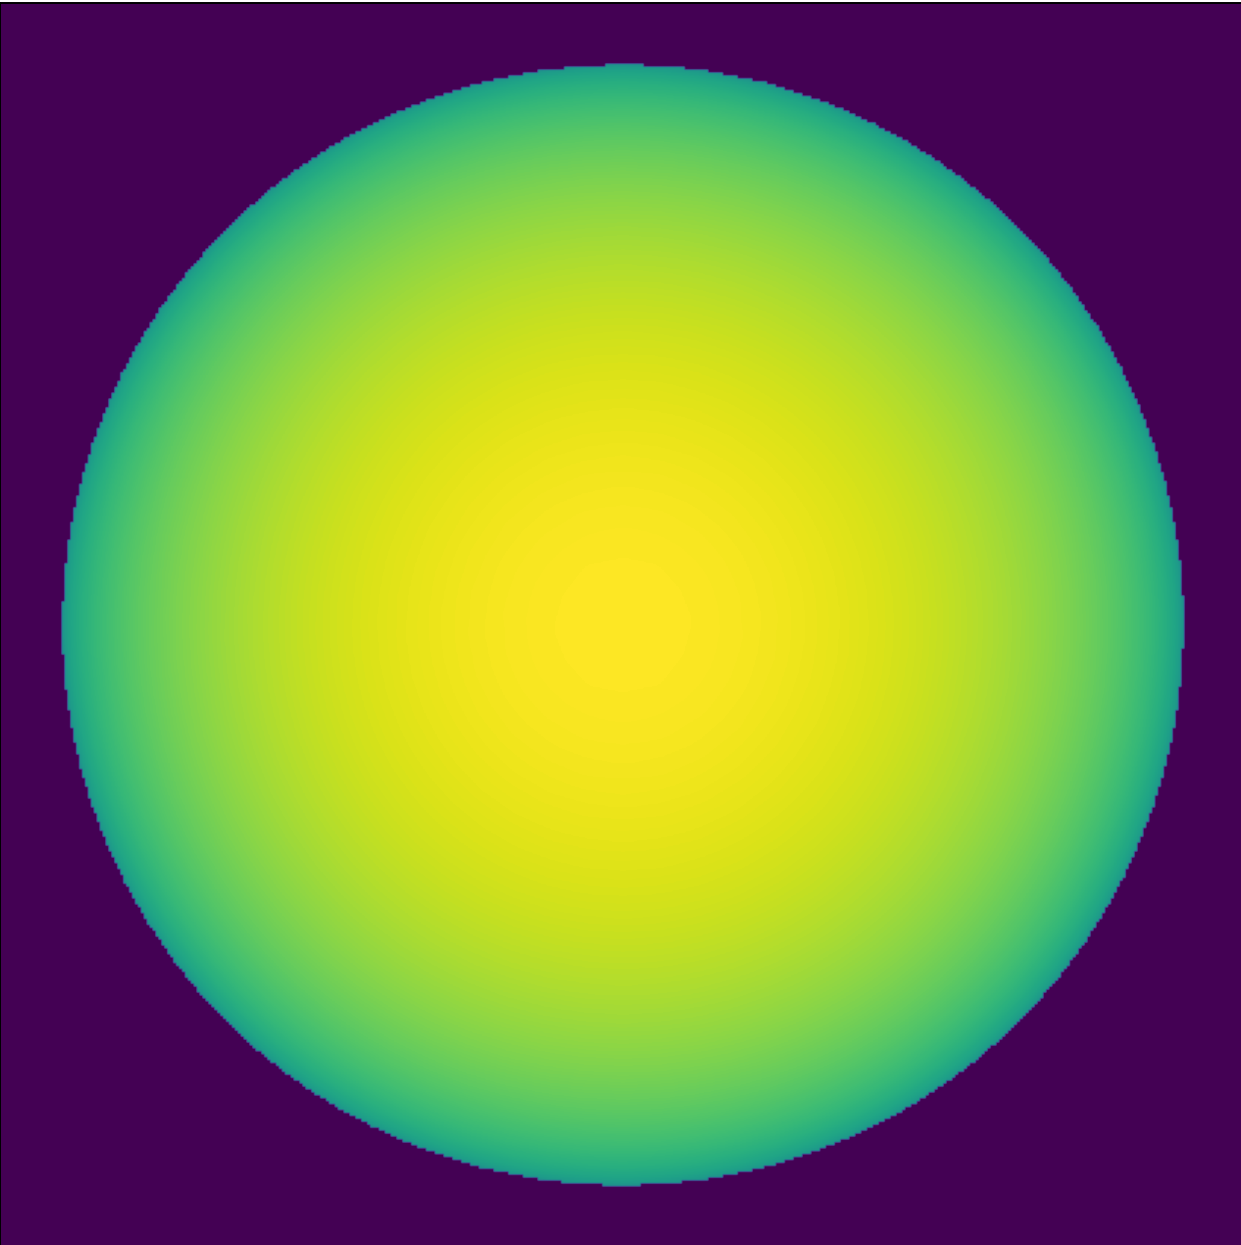
\includegraphics[width=.95\textwidth]{./immagini/sfera_singola.png}
        \caption{}
        \label{fig:sphere_a}
    \end{subfigure}
    \hfill
    \begin{subfigure}[b]{0.32\textwidth}
        % sfera_doppia
        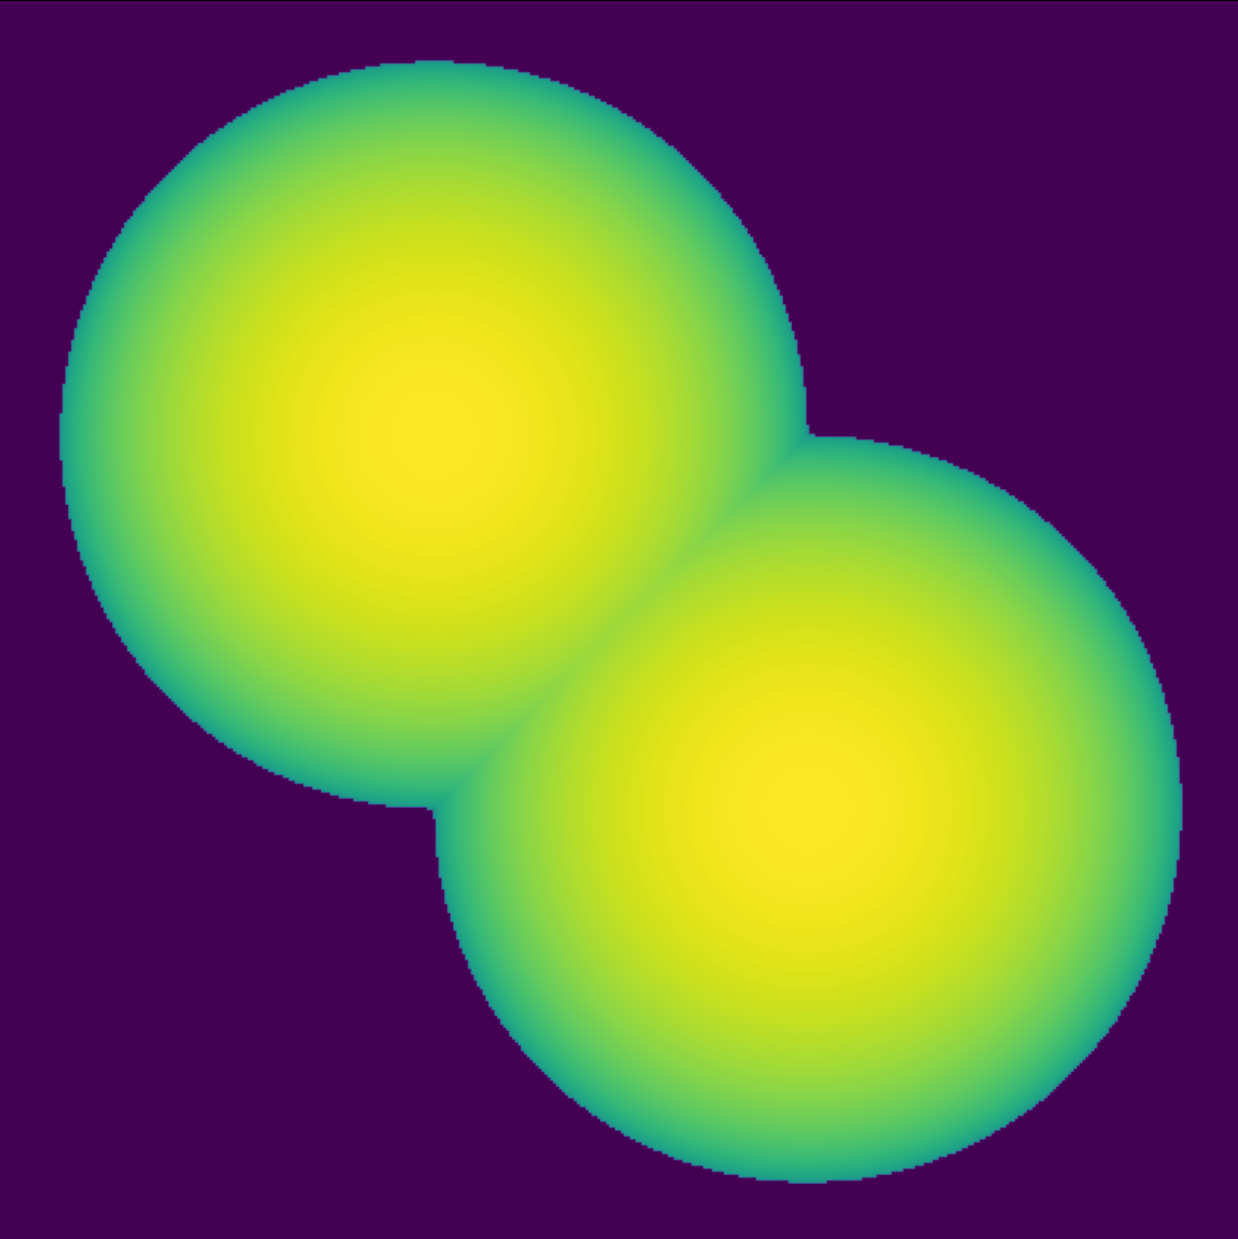
\includegraphics[width=.95\textwidth]{./immagini/sfera_doppia.png}
        \caption{}
        \label{fig:sphere_b}
    \end{subfigure}
    \hfill
    \begin{subfigure}[b]{0.32\textwidth}
        % sfera_statistica
        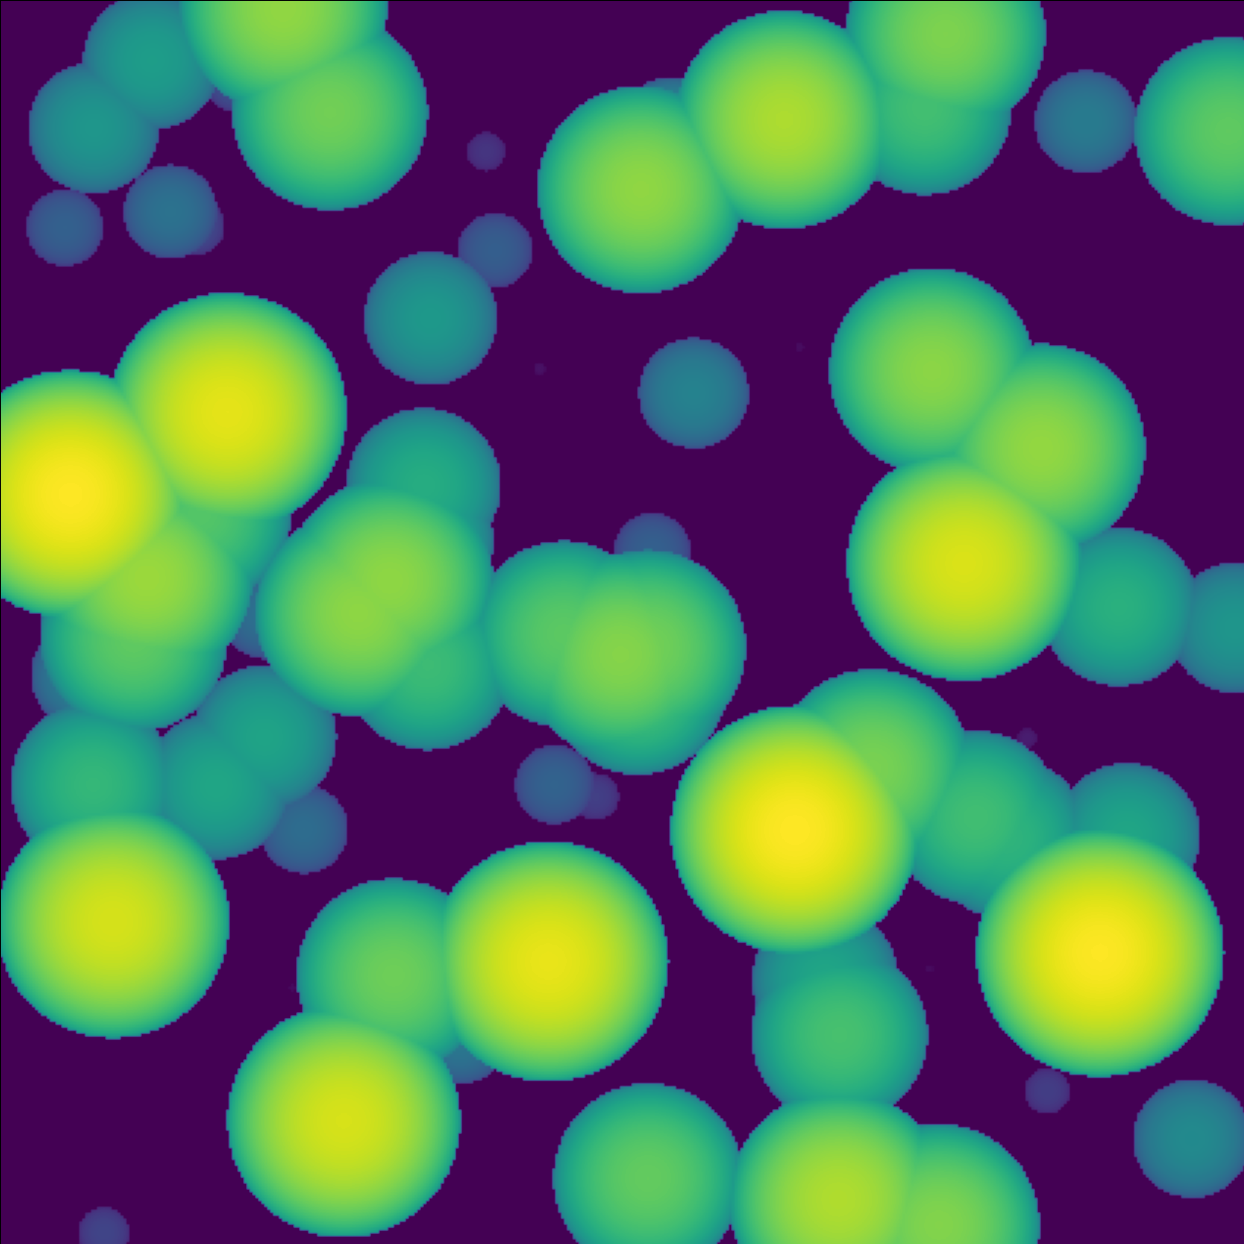
\includegraphics[width=.95\textwidth]{./immagini/sfera_statistica.png}
        \caption{}
        \label{fig:sphere_c}
    \end{subfigure}
    \caption{a) Single, b) Double and  c) Statistic used spheres}
    \label{fig:sphere}
\end{figure}

\newpage

\section{Nanosheets}

\paragraph{Creation process: }

The standard model is created in Blender using a cube with a central subdivision along the Y axis. It is centred in the origin with half size equal to 1. The geometrical shape of a nanosheet is well defined \cite{angleTIO2} with an angle of 68.3° obtained from anatase $TiO_2$ X-ray measurements. This recurring feature gives us the possibility to generate a standard, unitary-sized, model to use as a template for all the future instances.
The final model is obtained after a series of steps applied to the template model, as shown in Fig. \ref{fig:nano_creation}:
%
\begin{itemize}
    \item Scale along Y axis (to match the correct ratio between height and width) equals to: $S_Y = h / w$
    \item Scale along XZ plane (to generate the insets of the superior and inferior faces) equals to: $S_{XZ} = 1 - (h_{\text{eff}} / tan(68.3^{\circ}))$
\end{itemize}
%
Where h\_eff is the new calculated height.

\begin{figure}[ht]
    \centering
    \begin{subfigure}[b]{0.3\textwidth}
        % nano_1_1
        \includegraphics[width=.95\textwidth]{./immagini/nano_1_1.png}
        \caption{}
        \label{fig:nano_creation_a}
    \end{subfigure}
    \hfill
    \begin{subfigure}[b]{0.3\textwidth}
        % nano_1_2
        \includegraphics[width=.95\textwidth]{./immagini/nano_1_2.png}
        \caption{}
        \label{fig:nano_creation_b}
    \end{subfigure}
    \hfill
    \begin{subfigure}[b]{0.3\textwidth}
        % nano_1_3
        \includegraphics[width=.95\textwidth]{./immagini/nano_1_3.png}
        \caption{}
        \label{fig:nano_creation_c}
    \end{subfigure}
    \caption{Creation of steps: a) Scale along Y axis, b) Inset of the superior and inferior surfaces c) Final standard model}
    \label{fig:nano_creation}
\end{figure}

\paragraph{Positioning process: }

The additional information provided enables us to execute additional steps. This will include passages such as: floor process, positioning, rotation and scale, as shown in Fig. \ref{fig:nano_pos}:


\begin{itemize}
    \item The standard model is centered in the world origin, this means that we need to floor it (position the model so it will not clip with the floor substrate).
    \item Given the different size of the particle can be scaled accordingly, remembering that the half size of the standard model is equal to 1. This means we need to scale everything by a factor of (nominal\_size / 2).
    \item Now that the particle is generated and resized it now possible to traslate it by a vector $\vec{v}$ = (x, z) on the floor.
\end{itemize}

\begin{figure}[ht]
    \centering
    \begin{subfigure}[b]{0.3\textwidth}
        % nano_2_1
        \includegraphics[width=.95\textwidth]{./immagini/nano_2_1.png}
        \caption{}
        \label{fig:nano_pos_a}
    \end{subfigure}
    \hfill
    \begin{subfigure}[b]{0.3\textwidth}
        % nano_2_2
        \includegraphics[width=.95\textwidth]{./immagini/nano_2_2.png}
        \caption{}
        \label{fig:nano_pos_b}
    \end{subfigure}
    \hfill
    \begin{subfigure}[b]{0.3\textwidth}
        % nano_2_3
        \includegraphics[width=.95\textwidth]{./immagini/nano_2_3.png}
        \caption{}
        \label{fig:nano_pos_c}
    \end{subfigure}
    \caption{Creation of steps: a) Scale along Y axis, b) Inset of the superior and inferior surfaces c) Final standard model}
    \label{fig:nano_pos}
\end{figure}

\newpage

\paragraph{Examples: }

Some examples of generated images are reported in Fig. \ref{fig:nanosheet}a-c. In particular, Fig. \ref{fig:nanosheet_b} and \ref{fig:nanosheet_c} show compenetrated nanosheets, that are successfully handled by this system.

\begin{figure}[ht]
    \centering
    \begin{subfigure}[b]{0.3\textwidth}
        % nanosheet_singola
        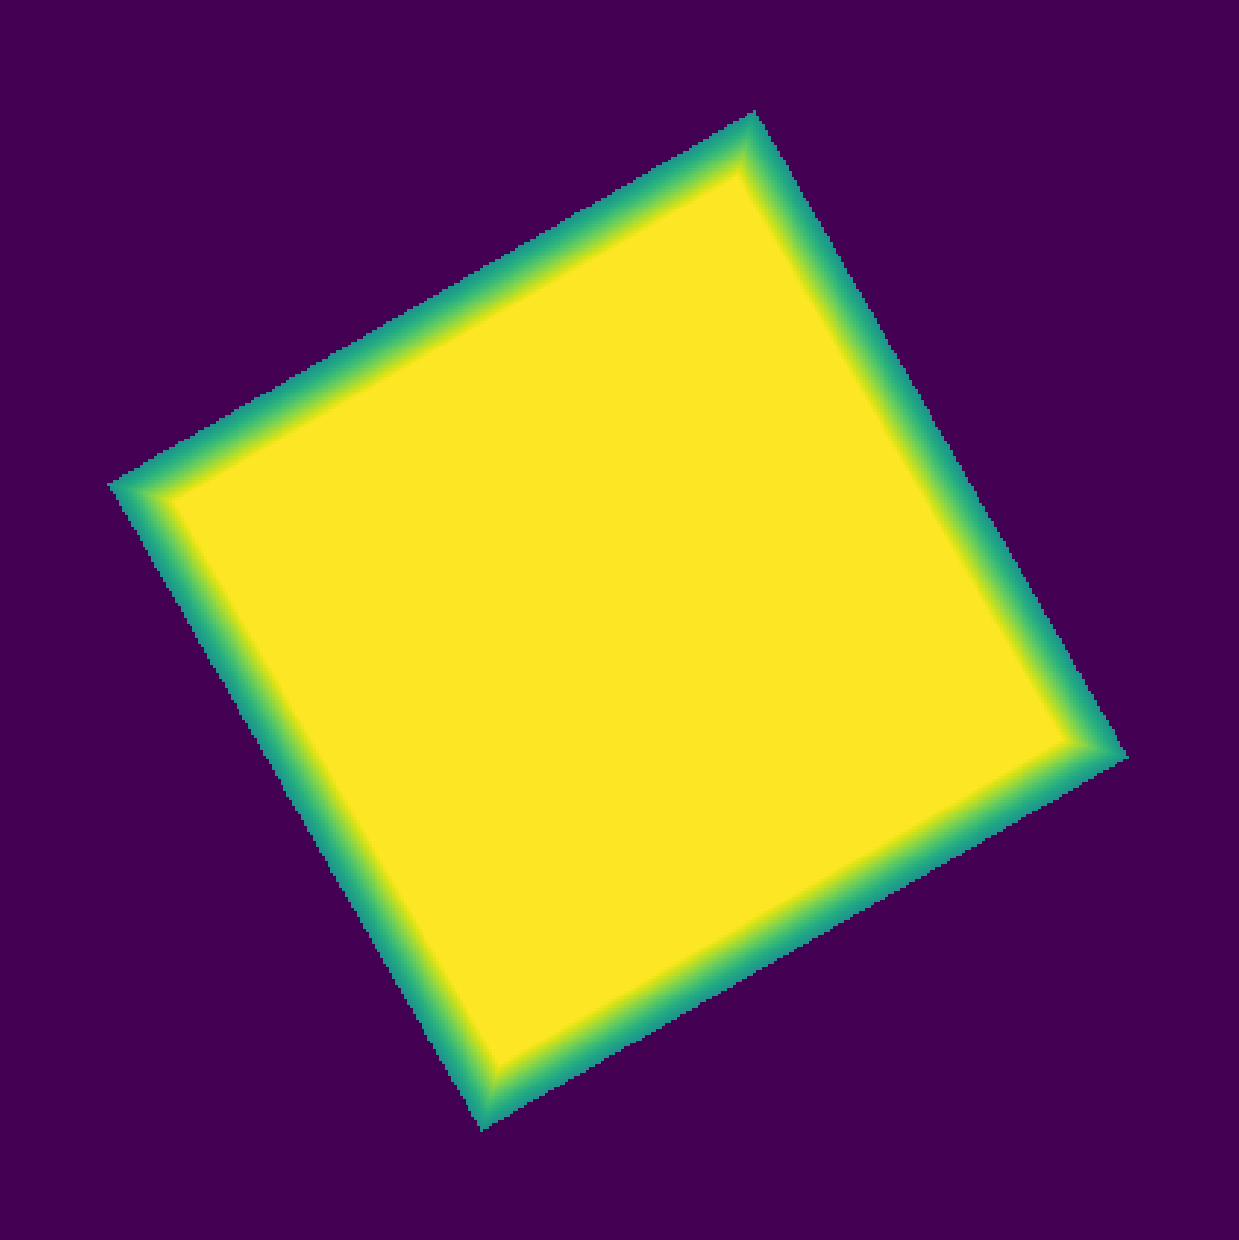
\includegraphics[width=.95\textwidth]{./immagini/nanosheet_singola.png}
        \caption{}
        \label{fig:nanosheet_a}
    \end{subfigure}
    \hfill
    \begin{subfigure}[b]{0.3\textwidth}
        % nanosheet_doppia
        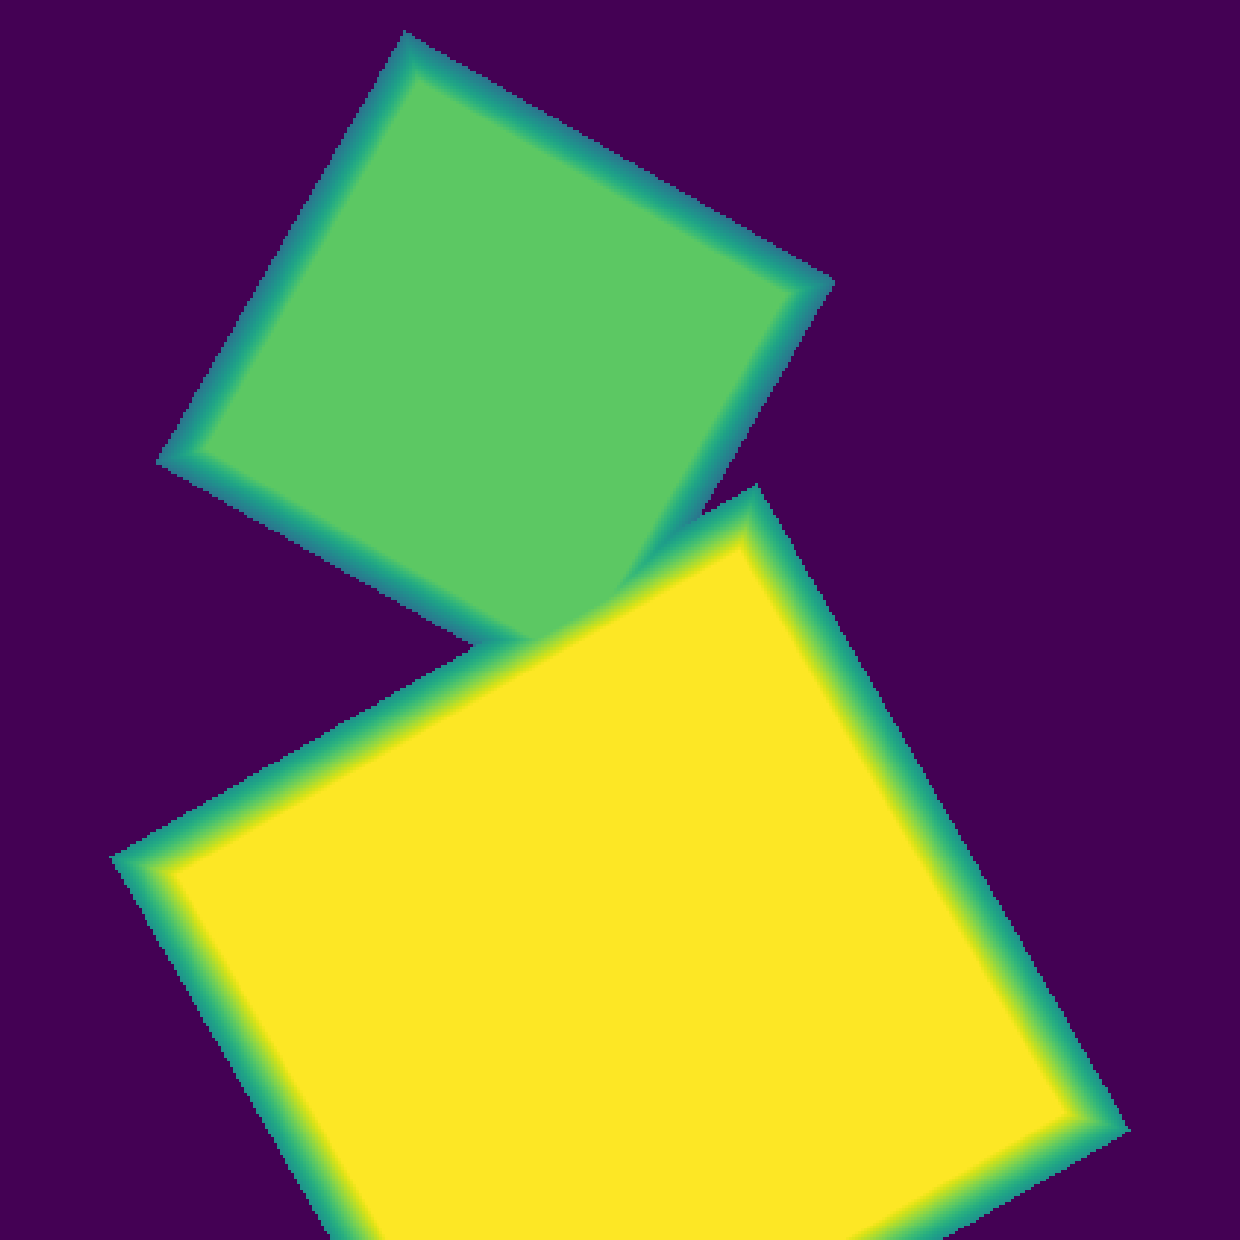
\includegraphics[width=.95\textwidth]{./immagini/nanosheet_doppia.png}
        \caption{}
        \label{fig:nanosheet_b}
    \end{subfigure}
    \hfill
    \begin{subfigure}[b]{0.3\textwidth}
        % nanosheet_statistica
        
\includegraphics[width=.95\textwidth]{./immagini/nanosheet_statistica.png}
        \caption{}
        \label{fig:nanosheet_c}
    \end{subfigure}
    \caption{a) Single, b) Double and  c) Statistic used nanosheets}
    \label{fig:nanosheet}
\end{figure}

\newpage

\section{Bipyramids}

\paragraph{Creation process: }

The whole process is very similar to the nanosheets one. The key difference is that the model becomes taller therefore more unstable. It will be necessary to lay the bipyramid down on one side. This is not a fixed rule, but statistically it's more common to find the nanoparticle on it's more stable equilibrium.

The standard model is created in Blender using a cube with a central subdivision along the Y axis. It is centered in the origin with half size equal to 1.

Several other passages are applied in order to obtain the correct model to use later, as shown in Fig. \ref{fig:bipyramids_process}:

\begin{itemize}
    \item Scale along Y axis (to match the correct ratio between height and width) equals to: $S_Y = h / w$
    \item Scale along XZ plane (to generate the insets of the superior and inferior faces) equals to: $S_{XZ} = 1 - (h_{eff} / tan(68.3^{\circ}))$
\end{itemize}

Where h\_eff is the new calculated height and $68.3^{\circ}$ is the crystalline angle of anatase $TiO_2$ from X-ray measurements.

\begin{figure}[ht]
    \centering
    \begin{subfigure}[b]{0.3\textwidth}
        % bipi_1_1
        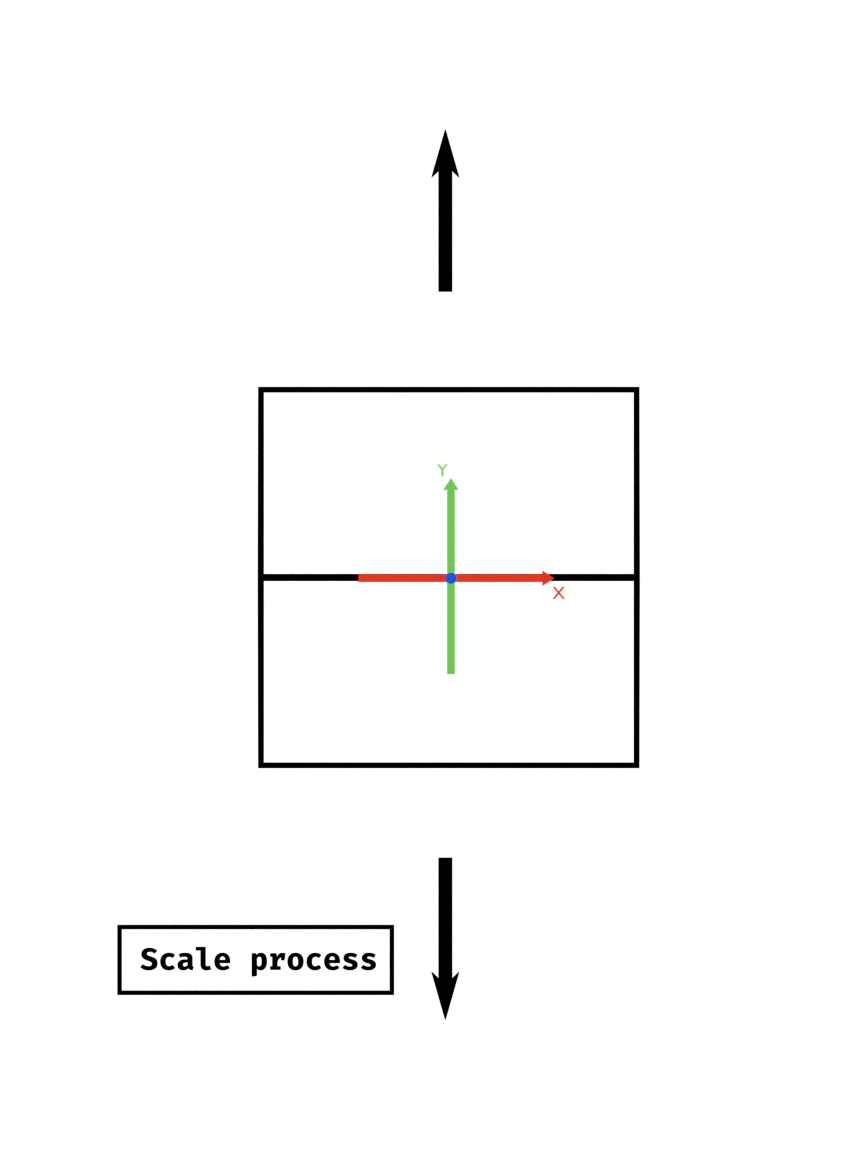
\includegraphics[width=.95\textwidth, clip]{./immagini/bipi_1_1.png}
        \caption{}
        \label{fig:bipyramids_process1}
    \end{subfigure}
    \hfill
    \begin{subfigure}[b]{0.3\textwidth}
        % bipi_1_2
        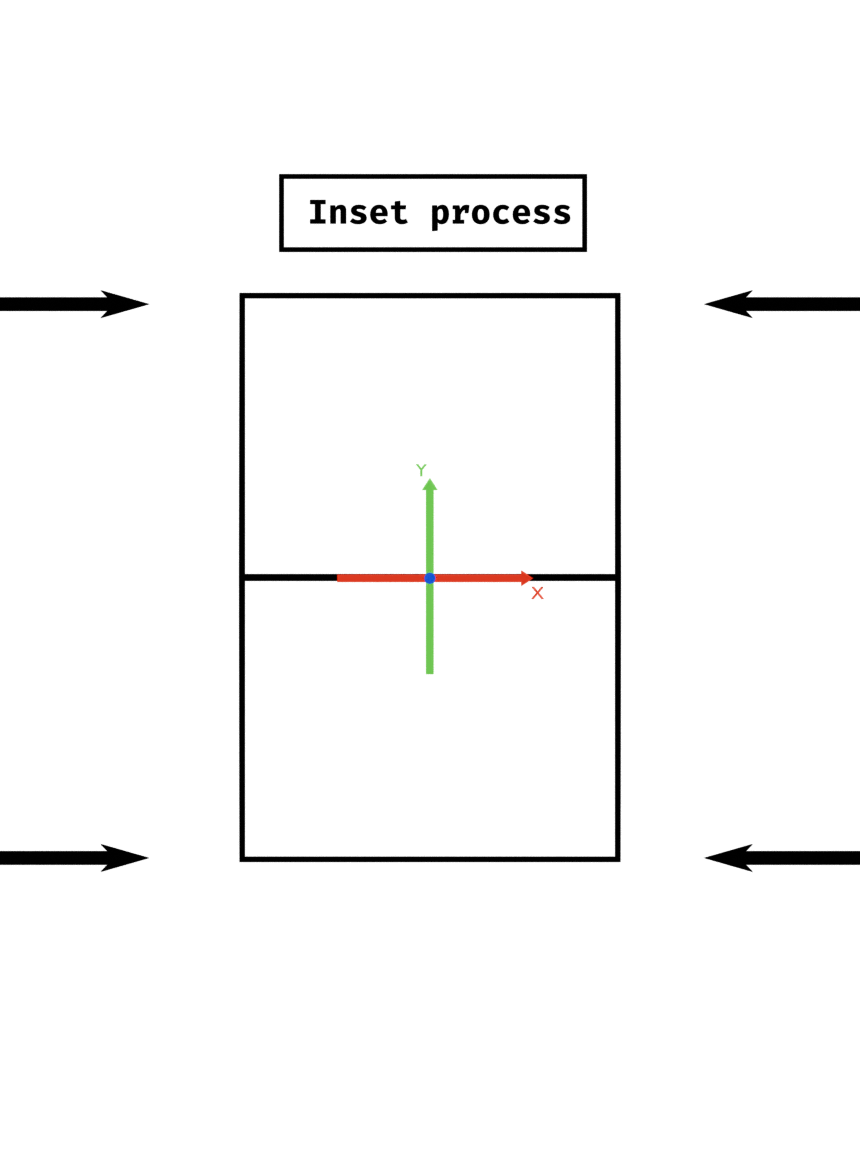
\includegraphics[width=.95\textwidth, clip]{./immagini/bipi_1_2.png}
        \caption{}
        \label{fig:bipyramids_process2}
    \end{subfigure}
    \hfill
    \begin{subfigure}[b]{0.3\textwidth}
        % bipi_1_3
        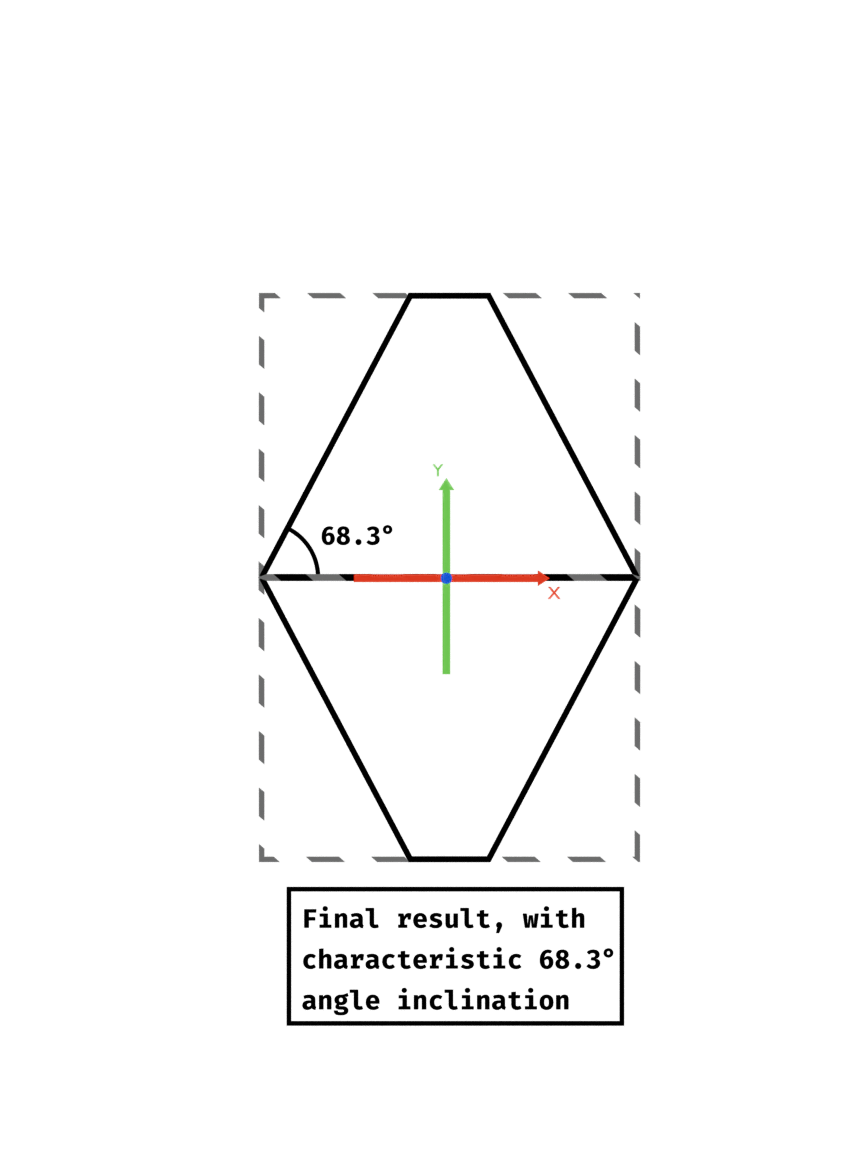
\includegraphics[width=.95\textwidth, clip]{./immagini/bipi_1_3.png}
        \caption{}
        \label{fig:bipyramids_process3}
    \end{subfigure}
    \caption{Creation steps: a) Scale along Y axis b) inset of the superior and inferior surfaces c) final standard model}
    \label{fig:bipyramids_process}
\end{figure}

\paragraph{Positioning process: }

After that, it must be positioned onto one of the diagonal faces, since the small bottom base will not ensure the maximum equilibrium. This is done by moving along the Y axis the model, so that the bottom base sits on the floor. Subsequently, a rotation matrix along the X axis is applied to rotate the bipyramid of $68.3^{\circ}$, as shown in Fig. \ref{fig:bipyramids_positioning}:

\begin{figure}[ht]
    \centering
    \begin{subfigure}[b]{0.22\textwidth}
        % bipi_2_1
        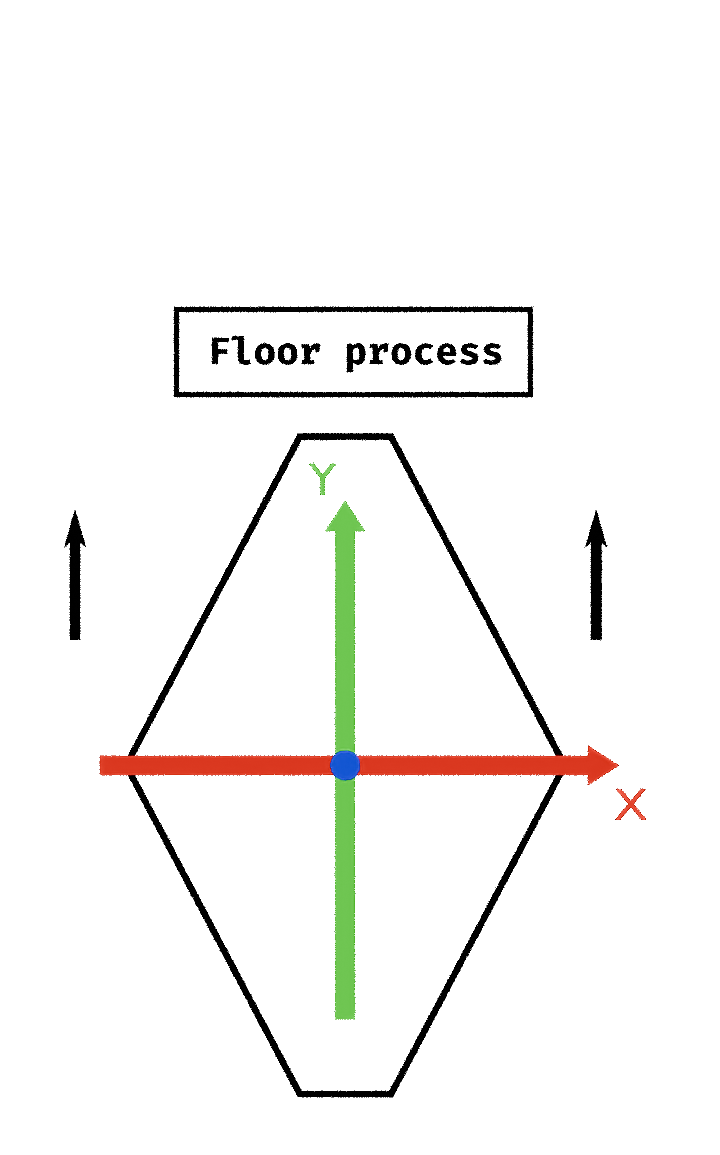
\includegraphics[width=.95\textwidth, clip]{./immagini/bipi_2_1.png}
        \caption{}
        \label{fig:bipyramids_positioning1}
    \end{subfigure}
    \hfill
    \begin{subfigure}[b]{0.22\textwidth}
        % bipi_2_2
        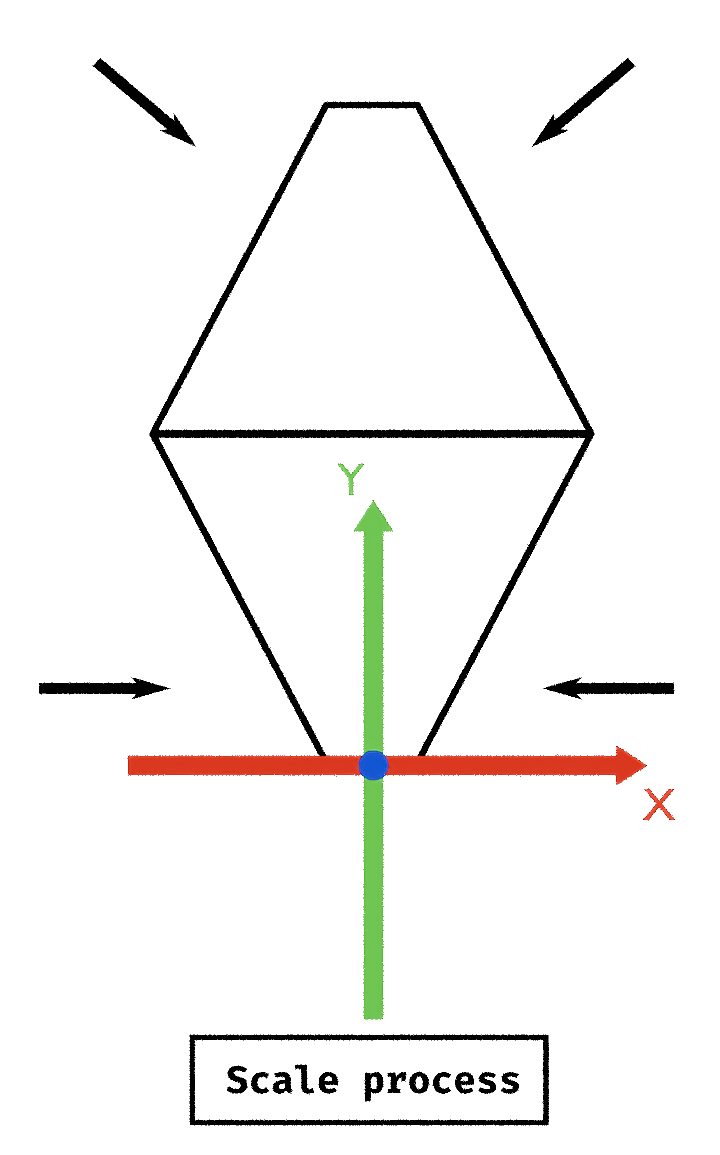
\includegraphics[width=.95\textwidth, clip]{./immagini/bipi_2_2.png}
        \caption{}
        \label{fig:bipyramids_positioning2}
    \end{subfigure}
    \hfill
    \begin{subfigure}[b]{0.22\textwidth}
        % bipi_2_3
        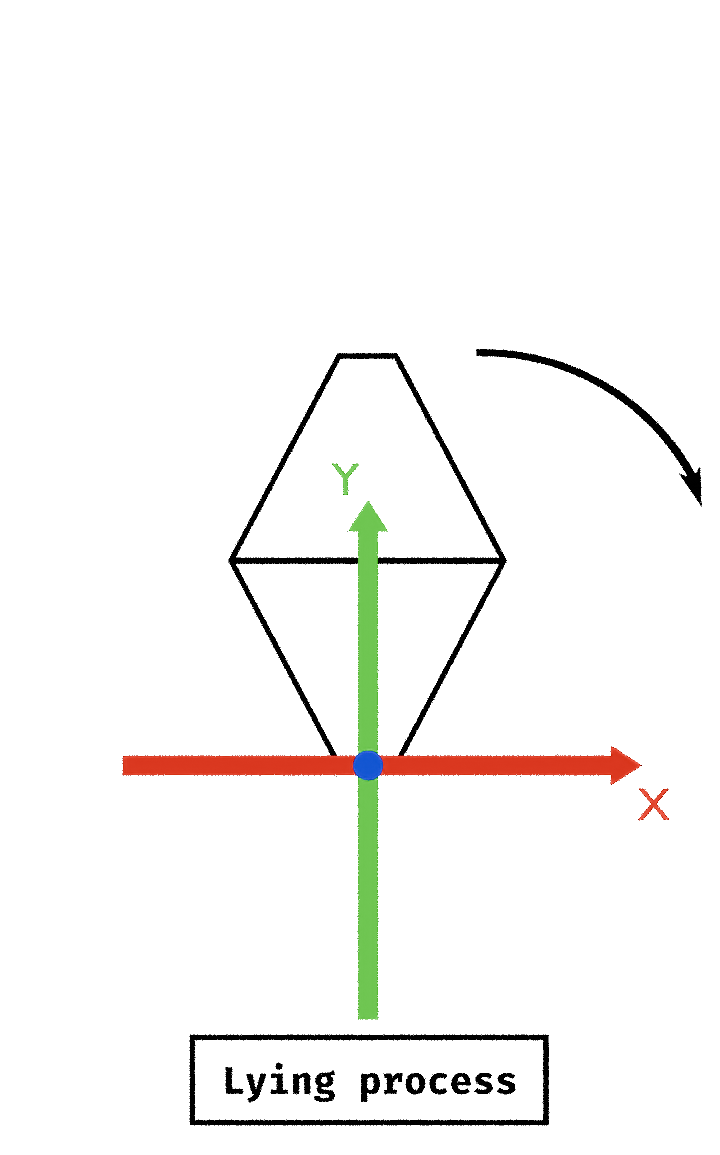
\includegraphics[width=.95\textwidth, clip]{./immagini/bipi_2_3.png}
        \caption{}
        \label{fig:bipyramids_positioning3}
    \end{subfigure}
    \hfill
    \begin{subfigure}[b]{0.22\textwidth}
        % bipi_2_4
        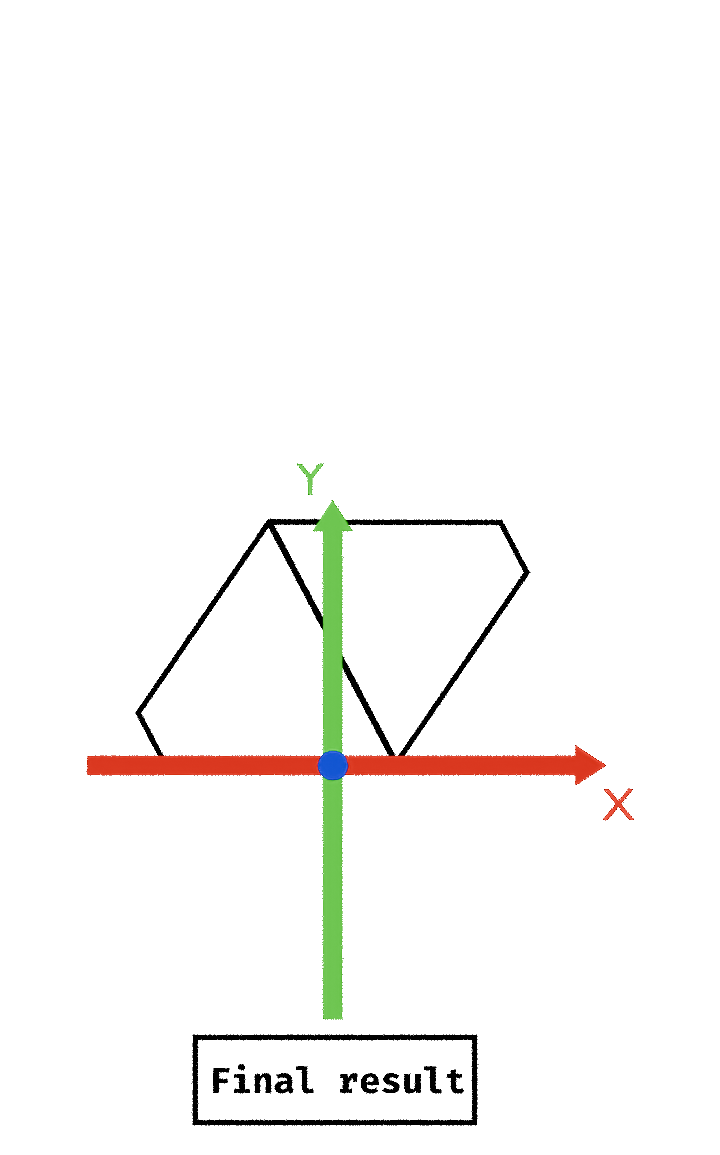
\includegraphics[width=.95\textwidth, clip]{./immagini/bipi_2_4.png}
        \caption{}
        \label{fig:bipyramids_positioning4}
    \end{subfigure}
    \caption{Instance positioning: a) floor process b) scaling process c) lying process d) final positioned model}
    \label{fig:bipyramids_positioning}
\end{figure}


\newpage

Finally, a traslation is applied in order to center the model on its center of mass. Thus, it will be easier for the user to position and rotate the desired nanoparticles on the substrate.

\paragraph{Examples: }

Some example of generated images are reported in Fig. \ref{fig:bipiramid_type} a-c. In particular, Fig. \ref{fig:bipiramid2} and \ref{fig:bipiramid3} shown also compenetrated nanosheets that are successfully handled by this system.

\begin{figure}[ht]
    \centering
    \begin{subfigure}[b]{0.3\textwidth}
        % bipiramid_singola
        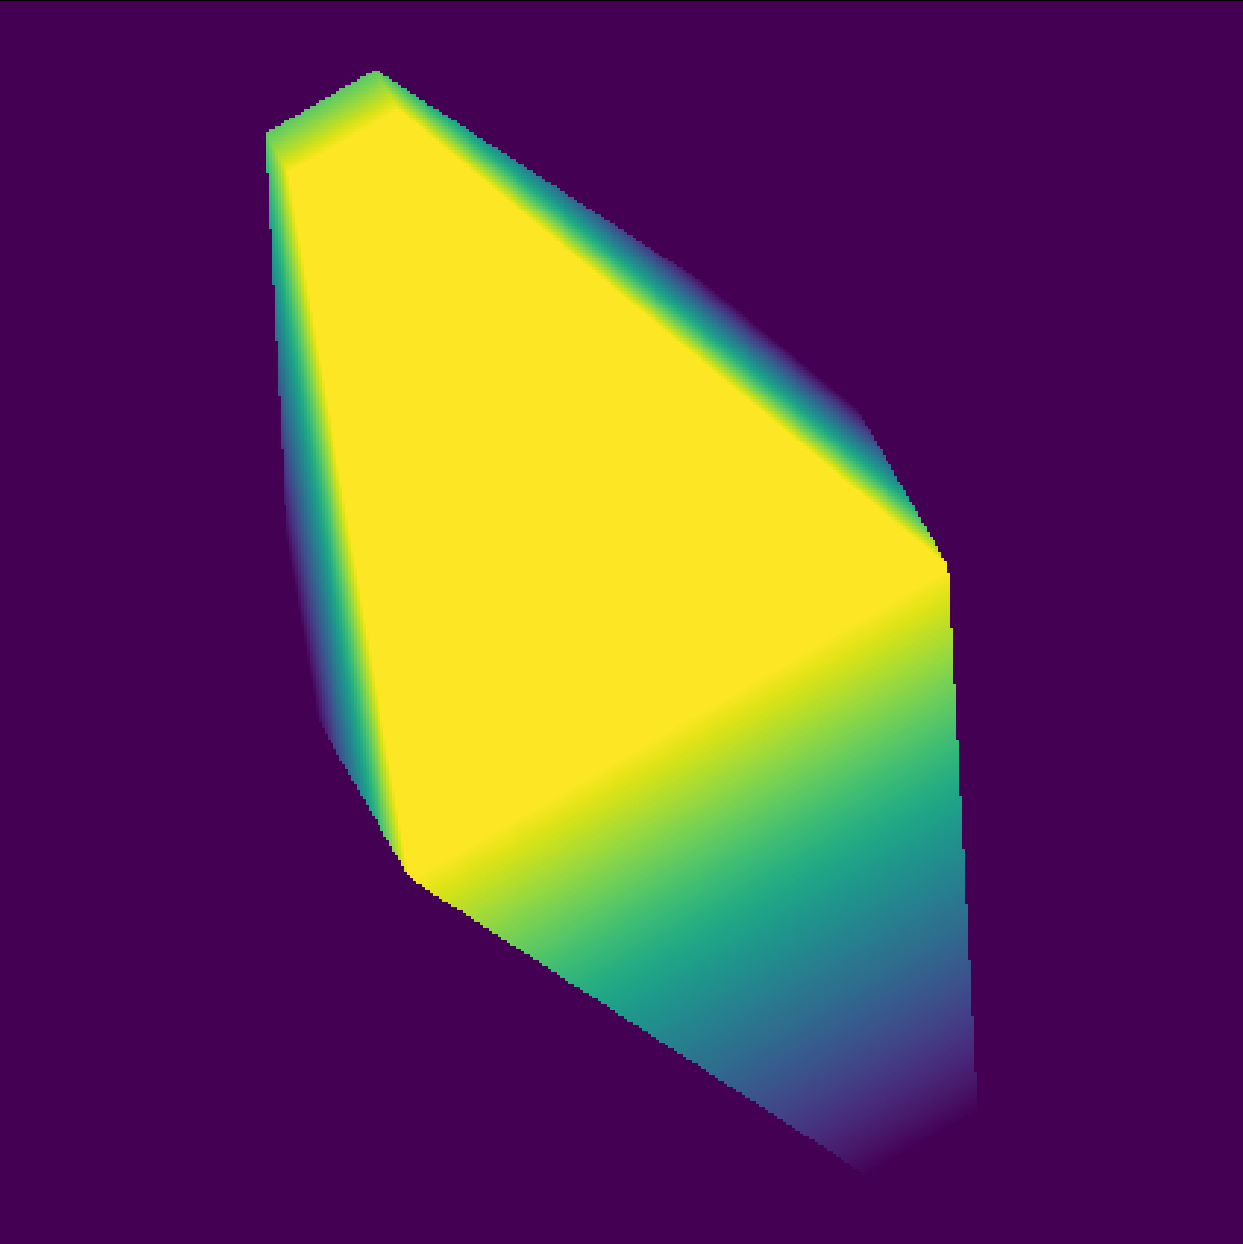
\includegraphics[width=.95\textwidth]{./immagini/bipiramid_singola.png}
        \caption{}
        \label{fig:bipiramid1}
    \end{subfigure}
    \hfill
    \begin{subfigure}[b]{0.3\textwidth}
        % bipiramid_doppia
        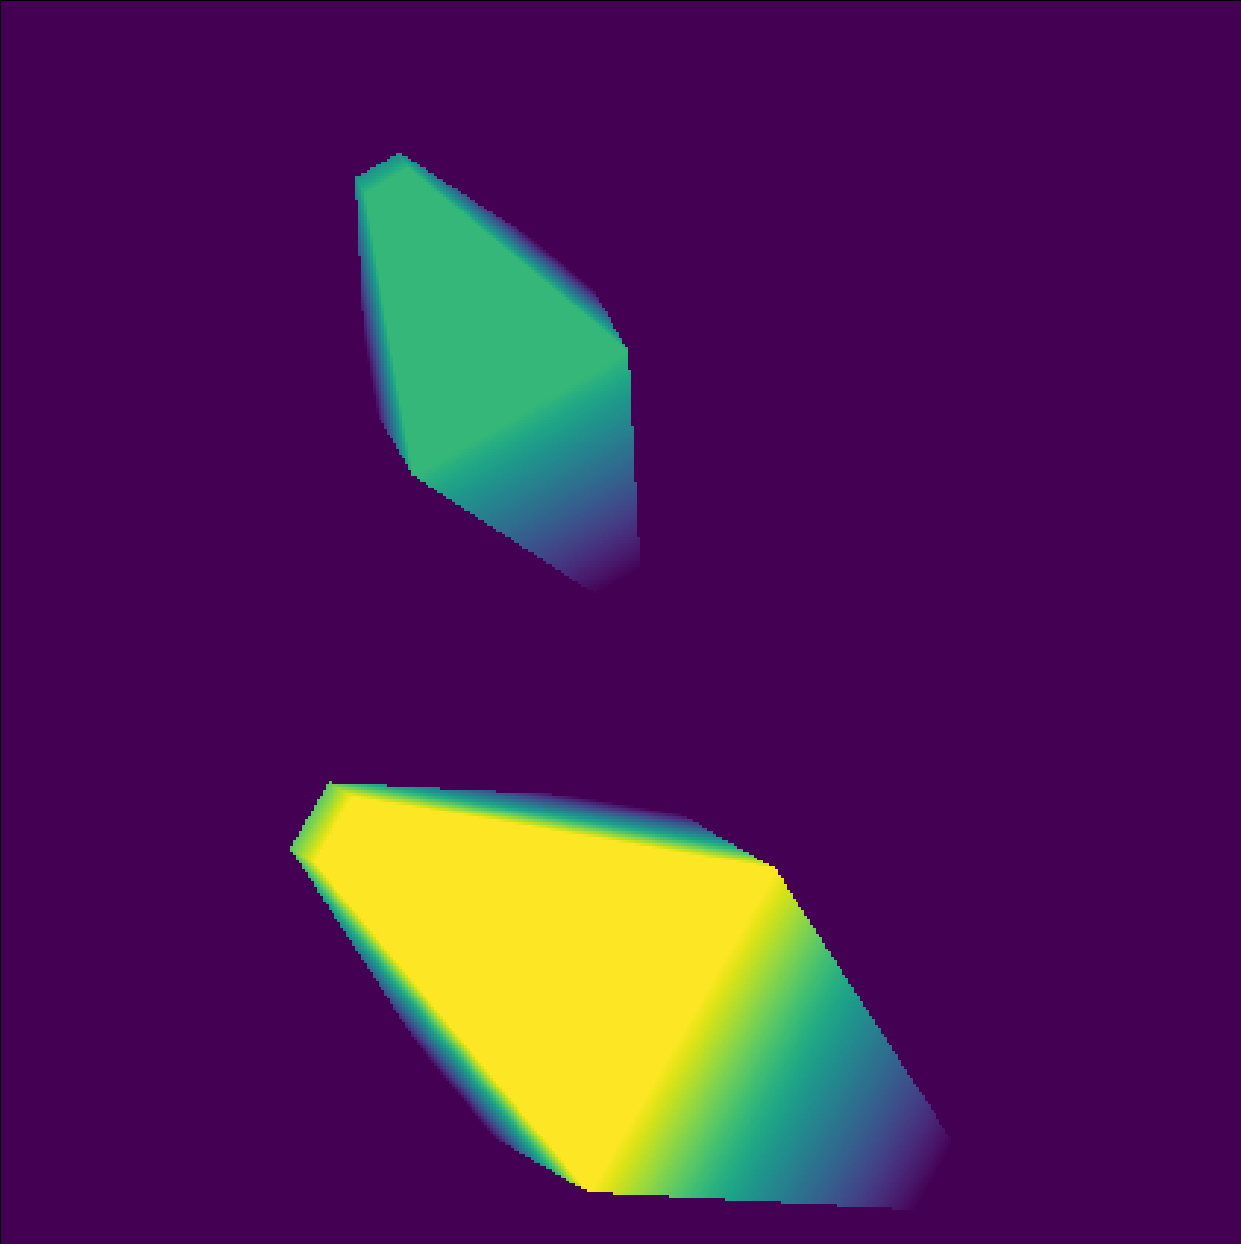
\includegraphics[width=.95\textwidth]{./immagini/bipiramid_doppia.png}
        \caption{}
        \label{fig:bipiramid2}
    \end{subfigure}
    \hfill
    \begin{subfigure}[b]{0.3\textwidth}
        % bipiramid_statistica
        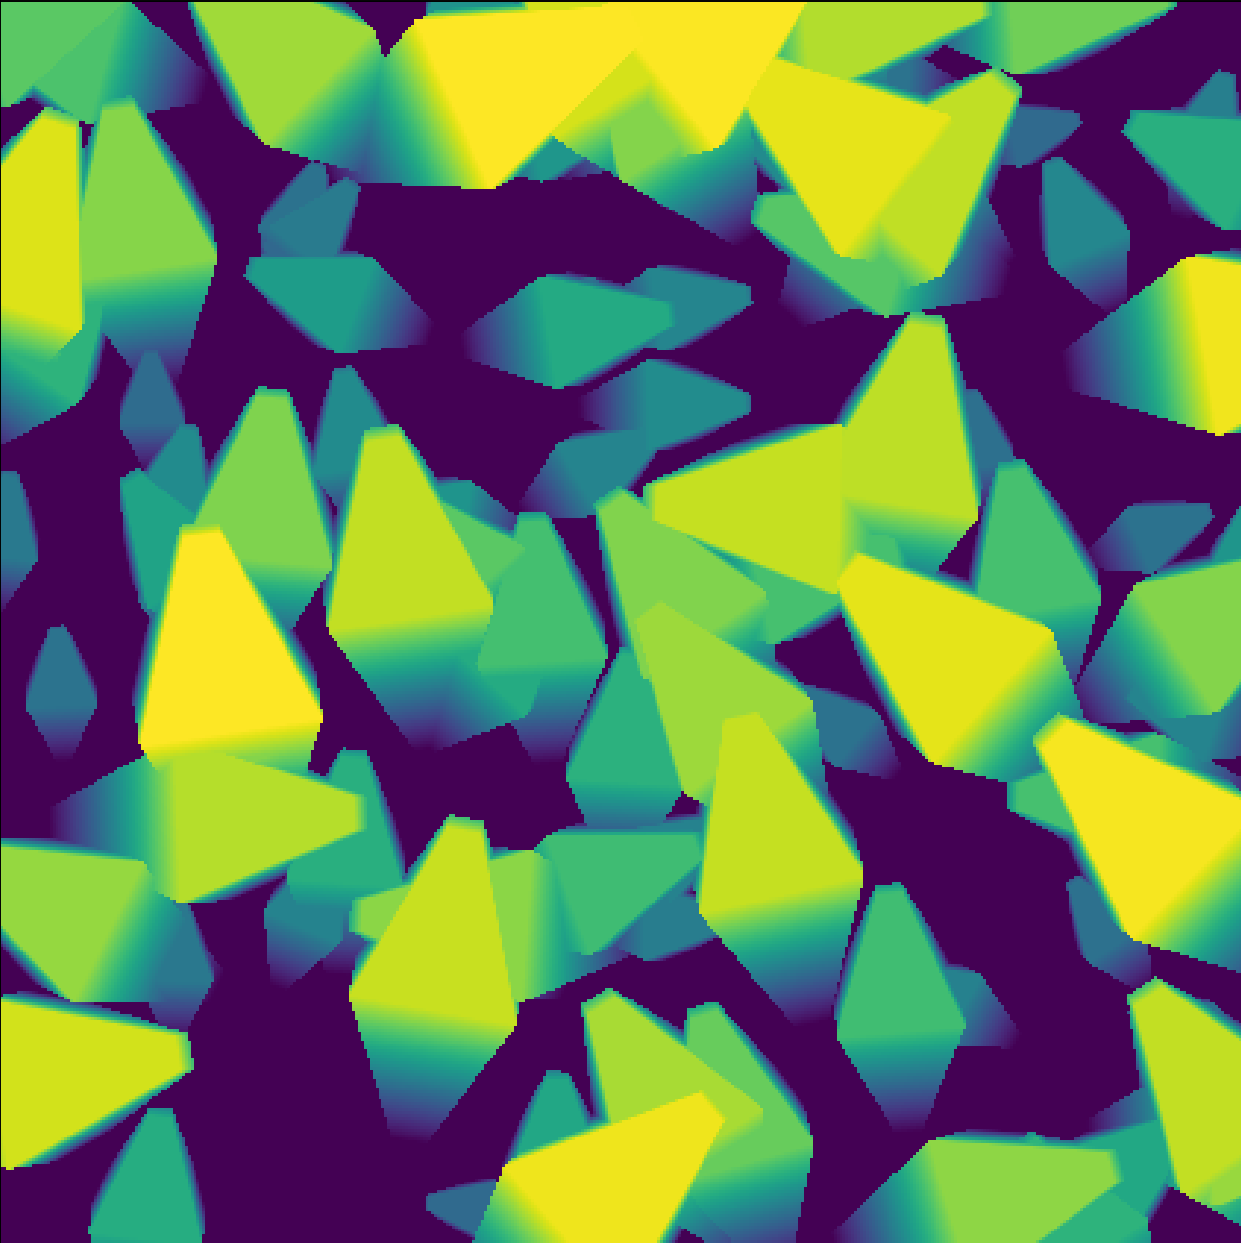
\includegraphics[width=.95\textwidth]{./immagini/bipiramid_statistica.png}
        \caption{}
        \label{fig:bipiramid3}
    \end{subfigure}
    \caption{Example of usage of bipiramids: a) Single b) Double c) Statistic}
    \label{fig:bipiramid_type}
\end{figure}
